% Shared by main.tex and supplemental_material.tex, so the two cannot drift
% apart in packages, theorem counters, colours or notation.
\documentclass[11pt]{article}

\usepackage[T1]{fontenc}
\usepackage[utf8]{inputenc}
\usepackage{lmodern}
\usepackage{microtype}

\usepackage{arxiv}

\usepackage{amsmath}
\usepackage{amssymb}
\usepackage{amsthm}
\usepackage{booktabs}
\usepackage{graphicx}
\usepackage{algorithm}
% `noend`: one-line bodies dominate here, and an explicit terminator after each
% of them costs more clarity than it buys. Indentation carries the structure.
\usepackage[noend]{algpseudocode}
\usepackage{tikz}
\usetikzlibrary{arrows.meta, positioning, fit, backgrounds, calc, patterns}
\usepackage{xcolor}
\usepackage[numbers,sort&compress]{natbib}
% Bibliography URLs are long enough to leave an underfull line if they can only
% break at punctuation; xurl lets them break anywhere.
\usepackage[hidelinks]{hyperref}
\usepackage{xurl}
\usepackage[capitalise,noabbrev]{cleveref}

% Each environment gets its own counter. Sharing one makes cleveref name every
% reference after the counter, so \cref of a definition comes out as "Theorem".
\theoremstyle{plain}
\newtheorem{theorem}{Theorem}
\newtheorem{proposition}{Proposition}
\theoremstyle{definition}
\newtheorem{definition}{Definition}
\theoremstyle{remark}
\newtheorem{remark}{Remark}

% The palette the figures were drawn with, so a TikZ schematic sitting beside
% one of them does not look like it came from a different document.
\definecolor{sccdTeal}{HTML}{0E8AA0}
\definecolor{sccdAmber}{HTML}{C07C10}
\definecolor{sccdPlum}{HTML}{8A3C74}
\definecolor{sccdMoss}{HTML}{3E6E4B}
\definecolor{sccdInk}{HTML}{333A41}
\definecolor{sccdGrid}{HTML}{D6DBE0}

% Notation used throughout, defined once.
\newcommand{\Fdiff}{\mathbf{F}}          % the difference function
\newcommand{\Rthree}{\mathbb{R}^{3}}
\newcommand{\toi}{t^{\star}}             % the reported time of impact
\newcommand{\toitrue}{\bar{t}}           % the true earliest root
\newcommand{\mach}{\varepsilon}          % machine epsilon
\newcommand{\dom}{\mathcal{B}}           % a box in (t, u, v)
\newcommand{\Cand}{\mathcal{C}}          % the candidate set
\newcommand{\Boxes}{\mathcal{B}}
\DeclareMathOperator{\hull}{hull}
% Small caps for the algorithm's named steps. Wrapped in \textnormal so it
% survives the italic body of a theorem, where lmodern has no italic small caps.
% The two primitives of a query and the quantity under test. These mark the role
% a term plays in an equation and set no colour: the formulas print black, and a
% reader who wants the correspondence with a schematic has the symbol names.
% They are kept as markup so the roles stay visible in the source and the
% typographic treatment can be changed in one place.
\newcommand{\primA}[1]{#1}
\newcommand{\primB}[1]{#1}
\newcommand{\tested}[1]{#1}

\newcommand{\op}[1]{\textnormal{\textsc{#1}}}

% Generated tables are as wide as their data. This shrinks one only when it
% would otherwise run into the margin, and leaves every table that already fits
% at its natural size -- so the common case keeps the body font exactly.
% Float placement. The defaults reserve so much of a page for text that a
% float-heavy document leaves gaps and pushes floats pages away from the prose
% that cites them. These let a float take more of a page and let a float page
% fill up before it is broken.
\renewcommand{\topfraction}{0.9}
\renewcommand{\bottomfraction}{0.8}
\renewcommand{\textfraction}{0.07}
\renewcommand{\floatpagefraction}{0.75}
\setcounter{topnumber}{3}
\setcounter{totalnumber}{4}

% The supplement is a separate document, so the article names it rather than
% \cref-ing into it; referencing both ways would make each need the other's aux.
% The silent-overflow finding, in one place. It is cited to its authors'
% benchmark, and it names a defect we intend to patch upstream, so it will want
% revising once that lands -- having it in a macro means revising it once.
\newcommand{\silentoverflow}{%
\citet{belgrod2025toi} benchmark thirteen broad-phase implementations against
exact ground truth and find that several of them \emph{miss collisions}, usually
through a fixed-size candidate buffer that discards overflow silently}

\newcommand{\supp}{the supplemental material}
\newcommand{\Supp}{The supplemental material}

\newcommand{\fittable}[1]{%
  \resizebox{\ifdim\width>\linewidth \linewidth\else \width\fi}{!}{#1}}


% Cross-document references into the paper, so a \cref here that names a section
% or an algorithm of the article resolves to the number the article gave it.
% Needs main.aux present, which `make supplemental` guarantees by building the
% article first.
\usepackage{xr-hyper}
\externaldocument{main}

\headertitle{Supplemental material}
\preprintmark{\textsc{Supplemental material}}

\title{Supplemental material for\\
       \emph{A Conservative and Tight Continuous Collision Detection Pipeline\\
       for GPU and multicore CPUs}}

\author{%
  Patrick Zulian
  \and David Belgrod
  \and Bolun Wang
  \and Zachary Ferguson
  \and Xin Zhao
  \and Marco Attene
  \and Daniele Panozzo
  \and Teseo Schneider%
}

\date{\today}

\begin{document}
\maketitle

This document holds the per-scene tables and the hardware-counter study that
support the article. Section and algorithm numbers prefixed with the article's
numbering refer to it. Nothing here is a separate experiment: every number comes
from the runs the article reports, and the regeneration commands are the ones
recorded in its availability section.

\tableofcontents

\section{Where the two processors spend their time}
\label{sec:parallel:limits}

\Cref{sec:parallel:why} of the paper explains the device's disadvantage in
structural terms; the hardware counters below identify the resource each
processor is short of.
\Cref{tab:counters} is Nsight Compute over the device search kernel and
\cref{tab:counters-host,tab:symbols} are \texttt{perf} on the host, six scenes
each, at the \op{Tight} mode and the shipped parameters.

\paragraph{Memory traffic.} The device is not short of bandwidth. Across the
six scenes the search moves between $0.8$ and $220\,\mathrm{MB}$ of dynamic
random-access memory (DRAM) traffic per launch, and never exceeds $1.2\%$ of
sustained DRAM peak. Arithmetic needs more care, because the natural measure of
it is the wrong one here. \Cref{tab:pipes} reports what the units are doing, and
\cref{tab:throughput} reports the throughput that matters here, candidate pairs
resolved per second. The cache hierarchy explains the quiet memory system. On
armadillo-rollers the kernel touches $63.9\,\mathrm{MB}$ of L1 sectors,
$20.3\,\mathrm{MB}$ of those reach L2, and only $2.3\,\mathrm{MB}$ reach DRAM. A
box is small, and its parent's corners are still resident when its children are
built.

\paragraph{Functional-unit utilisation.} The functional units are not idle; the
multiprocessor is. Two columns of \cref{tab:pipes} are normalised differently.
The pipe columns give each unit's share of its peak issue rate \emph{while the
multiprocessor is active}, and on that basis the double-precision pipe runs at
$18$ to $29\%$ of peak and the integer arithmetic logic unit (ALU) at $15$ to
$25\%$, close behind it on every scene. The \emph{SM} column is the whole
multiprocessor's share of peak over \emph{elapsed} time, and on the smallest
scene it is $2.25\%$. Pipes that issue at a quarter of peak when they have warps
to issue from do not limit this kernel, and cheaper arithmetic would not move
it.

The elapsed-time column also shows where the grid stops mattering. It climbs with
the launch size, from $2.25\%$ at $0.41$ waves per multiprocessor to $28.4\%$ at
$4.44$, and then stops: n-body and puffer-ball, at $333$ and $475$ waves, reach
$26.4\%$ and $28.6\%$. Four waves is enough to cover the device, and the hundred
after that buy nothing.

No flop rate is reported here. A rate against arithmetic peak is the figure of
merit for a dense kernel, whose work is fixed and whose only question is how
fast it can be pushed through, whereas the work of a branch-and-bound search is
not fixed and the whole design exists to do less of it. Corner inheritance in
\cref{alg:host} turns eight corner evaluations into four, and sharing a bound
across queries takes the search from about eleven boxes per query to roughly
one. Both cut the flop count, and both make the implementation better. An
implementation that raised its flop rate while returning the same answers would
be a worse one. The rate therefore carries no information about quality, and the
comparison against peak none about headroom. What we claim from the pipe columns
is narrower: no functional unit is saturated, so no functional unit is the
limit.

The instruction mix settles one more question, the kind of arithmetic the search
does. Integer thread-instructions run at $0.58$ to $0.95$ per double-precision
instruction, so the kernel does nearly as much integer work as floating-point
work. That integer work is the algorithm itself: stack indices, query
identifiers, depth counters, the barycentric validity test and the atomics of
\cref{alg:device}. A corner evaluation is double-precision work, and a box is
more than a corner evaluation. The load-store pipe never exceeds $8.1\%$, the
instruction-side counterpart of the quiet DRAM above.

\begin{figure}[htbp]
  \centering
  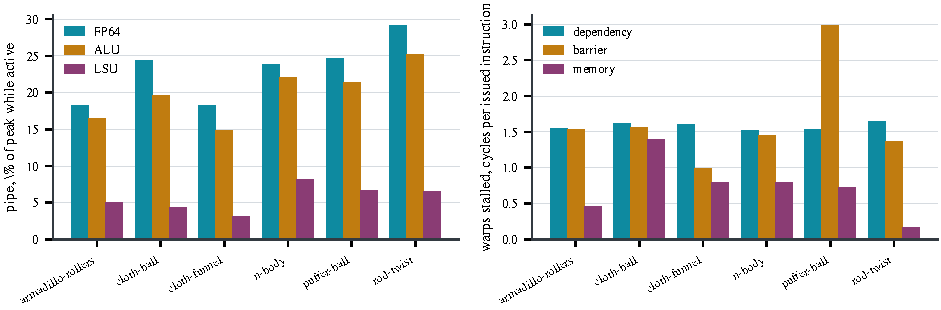
\includegraphics[width=\linewidth]{figures/device-counters.pdf}
  \caption{Device counters per scene. Left: each pipe's share of its peak issue
    rate while the multiprocessor is active. Right: warps stalled per issued
    instruction, by reason. The dependency term is flat across inputs whose
    launches differ by three orders of magnitude, which is the observation
    \cref{sec:parallel:limits} rests on. The tables are
    \cref{tab:pipes,tab:counters}.}
  \label{fig:counters}
\end{figure}

\paragraph{Available parallelism.} The kernel is not short of work to schedule
either, and six scenes establish this where two would not. The grid size spans
three orders of magnitude, from $0.41$ waves per multiprocessor on cloth-funnel,
where the launch does not cover the device even once, to $475$ on puffer-ball,
where it covers it hundreds of times over. Occupancy moves hardly at all across
that range, from $8.4\%$ to $16.3\%$, and the issue rate stays between $0.20$
and $0.35$ instructions per scheduler cycle out of a possible one. A kernel
short of parallelism would improve when handed four hundred times as much of it,
and this one does not.

\paragraph{Latency.} The limit is latency, and the same latency on every scene.
The last three columns of \cref{tab:counters} report the stall terms. Warps
stalled on an execution dependency sit between $1.52$ and $1.65$ on every scene,
a spread of $8\%$ across inputs whose launches differ by three orders of
magnitude in size and whose candidate pairs per step differ by a factor of seven
hundred. Stalls on memory are the smallest term almost everywhere, between
$0.17$ and $1.40$. A corner evaluation is a chain of dependent multiply--adds,
and with $8$ to $16\%$ of the warp slots filled, and $8$ to $24$ of a warp's
$32$ lanes doing useful work when an instruction issues, there are not enough
independent warps resident to cover that chain. Adding grid does not add
residency.

Barrier stalls are the one term that does move, from $0.99$ to $2.98$, with
puffer-ball at the top of that range. Three block-wide barriers per iteration
cost what the slowest thread in the block costs, and puffer-ball has both the
most candidate pairs per step and the widest spread of query difficulty. The
stall does not decide the outcome: puffer-ball's device narrow phase leads the
host by $16.51\times$ in \cref{tab:processor}, the largest such margin in the
benchmark. The counter bounds how much of that margin the barriers cost, and not
whether the device wins.

\paragraph{Host counters.} Grace is the opposite case. The host pipeline retires
between $2.8$ and $3.8$ instructions per cycle at an L1 data miss rate of $0.2$
to $2.1\%$, and the narrow phase on its own misses L1 on between $0.01$ and
$0.65\%$ of loads. The per-lane geometry replication of \cref{sec:parallel:host}
turns a gather into contiguous loads, and the counters show it doing so: a
lane's working set stays resident. Its instruction rate tracks how hard the
queries are and not how many there are. It is $0.49$ on cloth-ball, whose
searches are deep, against $2.87$ on n-body, where the median answer is within
$10^{-8}$ of the root and most queries are settled by a single box. That is the
same dependent chain the device stalls on, paid on a core with enough
out-of-order capacity to hide most of it.

\paragraph{Host costs outside the timings.} \Cref{tab:symbols} attributes
sampled host cycles to the object that spent them. On cloth-funnel $14.1\%$ of
them are inside \texttt{libm}, and the symbol profile puts all of that in one
call, the \texttt{pow} that raises $\delta$ to the third power in
\cref{eq:err}. The share is scene-dependent, falling to $2.6\%$ on
armadillo-rollers. It is written as \texttt{std::pow} deliberately.
\Cref{sec:prelim:err} records that the error bound is certified for one sequence
of operations, and the host keeps the reference's sequence so that its answers
stay bit-identical to it (\cref{sec:results:ref}). The device kernel does not
pay this cost, since it computes $\delta^{3}$ as a plain cube scaled to round
upward. The host could do the same, at the price of the exact agreement that
\cref{sec:results:ref} reports.

The OpenMP runtime is the second such cost, and at its worst it is the largest
of the three: $26.9\%$ of cycles on armadillo-rollers against $0.3\%$ on
puffer-ball. The ordering follows case count and not problem size.
Armadillo-rollers runs $781$ cases and puffer-ball $240$, and each case enters
and leaves the parallel regions of \cref{alg:cell,alg:cellmin} and the narrow
phase afresh. A scene made of many small steps therefore pays the runtime
repeatedly, whereas a scene made of few large ones amortises it away. SCCD's own
code accounts for the rest, between $45$ and $90\%$ of sampled cycles, depending
on how much of the profile the runtime and the operating system take.

\paragraph{Scope of the counters.} These counters cover one narrow-phase mode
and the earliest-impact kernel. The device figures are taken under a profiler
that serialises launches, so they support statements about ratios and none about
absolute time. The host rows are whole-process counters and not per-phase ones.
The pipeline row comes from a build with the device path compiled out, so it is
host work throughout; the narrow-phase row comes from the oracle, which also
drives the device modes, so its instruction rate is a floor. One prediction is
left untested, and it belongs to \cref{sec:parallel:device}: if idle threads
could claim new queries from a global cursor, the dependency and barrier stalls
should fall together. Nothing here confirms that they would.

\begin{table}[!tb]
  \centering
  \caption{Functional-unit use in the device search kernel. The first three
    columns are each pipe's share of its peak issue rate \emph{while the SM is
    active}; \emph{SM} is the whole multiprocessor's share of peak over
    \emph{elapsed} time, so the gap between them is the machine standing idle
    rather than the pipes running slowly. \emph{int/fp64} is integer
    thread-instructions per double-precision one. No flop rate is reported: the
    throughput figure for this pipeline is candidate pairs resolved per second
    (\cref{tab:throughput}), and an implementation that raised its arithmetic
    rate while returning the same answers would be a worse one.}
  \label{tab:pipes}
  \begin{tabular}{lrrrrr}
    \toprule
    & \multicolumn{3}{c}{pipe, \% of peak while active}
      & \multicolumn{2}{c}{} \\
    \cmidrule(lr){2-4}
    scene & FP64 & ALU & LSU & SM \% & int/fp64 \\
    \midrule
    armadillo-rollers & 18.3 & 16.5 & 5.0 & 4.89 & 0.77 \\
    cloth-ball & 24.3 & 19.6 & 4.4 & 4.03 & 0.71 \\
    cloth-funnel & 18.3 & 14.8 & 3.1 & 2.25 & 0.58 \\
    n-body & 23.8 & 22.0 & 8.1 & 26.37 & 0.95 \\
    puffer-ball & 24.6 & 21.4 & 6.7 & 28.61 & 0.90 \\
    rod-twist & 29.1 & 25.2 & 6.6 & 28.43 & 0.72 \\
    \bottomrule
  \end{tabular}
  \par\smallskip\footnotesize Source: \texttt{benchmark/results/profile/}
\end{table}


\begin{table}[!tb]
  \centering
  \caption{Nsight Compute counters for the device narrow-phase kernel, \op{Tight}
    mode, at the shipped parameters. \emph{DRAM} is read and write together for
    one launch and the share of sustained peak bandwidth it represents;
    \emph{lanes} is how many of a warp's $32$ are doing useful work when an
    instruction issues; \emph{issue} is instructions per scheduler cycle out of a
    possible one; \emph{waves} is how many times the grid covers the device. The
    last three columns are warps stalled per issue-active cycle, by reason. A
    profiler serialises launches, so the ratios here are comparable with
    \cref{sec:results} and the absolute times are not.}
  \label{tab:counters}
  \fittable{%
\begin{tabular}{lrrrrrrrrr}
    \toprule
    & \multicolumn{2}{c}{DRAM} & \multicolumn{4}{c}{utilisation}
      & \multicolumn{3}{c}{warps stalled on} \\
    \cmidrule(lr){2-3}\cmidrule(lr){4-7}\cmidrule(lr){8-10}
    scene & MB & \% peak & occ.\ \% & lanes & issue & waves
          & depend. & barrier & memory \\
    \midrule
    armadillo-rollers & 2.28 & 0.085 & 9.0 & 10.2 & 0.20 & 2.24 & 1.55 & 1.54 & 0.46 \\
    cloth-ball & 3.28 & 0.360 & 14.0 & 10.9 & 0.28 & 1.38 & 1.62 & 1.56 & 1.40 \\
    cloth-funnel & 0.84 & 0.082 & 8.4 & 13.8 & 0.20 & 0.41 & 1.60 & 0.99 & 0.80 \\
    n-body & 139.61 & 1.215 & 16.0 & 24.4 & 0.34 & 332.64 & 1.52 & 1.45 & 0.79 \\
    puffer-ball & 219.68 & 1.102 & 16.3 & 18.3 & 0.30 & 475.46 & 1.54 & 2.98 & 0.73 \\
    rod-twist & 5.34 & 0.180 & 14.0 & 8.0 & 0.35 & 4.44 & 1.65 & 1.37 & 0.17 \\
    \bottomrule
  \end{tabular}}
  \par\smallskip\footnotesize Source: \texttt{benchmark/results/profile/}
\end{table}


\begin{table}[!tb]
  \centering
  \caption{\texttt{perf stat} counters on Grace. \emph{pipeline} is the whole
    host pipeline from a build with the device path compiled out, so it is host
    work throughout; \emph{narrow phase} is the accuracy oracle, which runs the
    narrow phase over the curated query sets and no broad phase at all. Both are
    whole-process counters.}
  \label{tab:counters-host}
  \begin{tabular}{lrrrr}
    \toprule
    & \multicolumn{2}{c}{pipeline} & \multicolumn{2}{c}{narrow phase} \\
    \cmidrule(lr){2-3}\cmidrule(lr){4-5}
    scene & inst/cycle & L1 miss \% & inst/cycle & L1 miss \% \\
    \midrule
    armadillo-rollers & 3.29 & 0.73 & 0.80 & 0.35 \\
    cloth-ball & 2.78 & 1.38 & 0.49 & 0.46 \\
    cloth-funnel & 3.35 & 1.31 & 0.84 & 0.55 \\
    n-body & 2.86 & 0.76 & 2.87 & 0.01 \\
    puffer-ball & 3.77 & 2.11 & 1.13 & 0.31 \\
    rod-twist & 3.13 & 0.23 & 0.87 & 0.65 \\
    \bottomrule
  \end{tabular}
  \par\smallskip\footnotesize Source: \texttt{benchmark/results/profile/}
\end{table}


\begin{table}[!tb]
  \centering
  \caption{Where the host spends its cycles, from a sampling profile of the
    CUDA-free build attributed by shared object. \emph{SCCD} is our own code,
    which inlines into the driver; \emph{OpenMP} is the runtime behind the
    parallel loops; \emph{libm} is almost entirely the call that raises $\delta$
    to the third power in \cref{eq:err}. The profile covers the whole process,
    so mesh loading and allocation are in it as well as the pipeline, which is
    most of what the last column holds.}
  \label{tab:symbols}
  \begin{tabular}{lrrrrr}
    \toprule
    scene & SCCD & OpenMP & libm & libc & kernel, other \\
    \midrule
    armadillo-rollers & 48.3 & 26.9 & 2.6 & 16.1 & 6.0 \\
    cloth-ball & 79.9 & 2.0 & 6.3 & 10.1 & 1.6 \\
    cloth-funnel & 44.9 & 6.6 & 14.1 & 3.6 & 30.8 \\
    n-body & 78.3 & 1.5 & 10.7 & 8.4 & 0.9 \\
    puffer-ball & 90.2 & 0.3 & 3.5 & 5.5 & 0.3 \\
    rod-twist & 66.4 & 4.9 & 2.1 & 2.4 & 24.1 \\
    \bottomrule
  \end{tabular}
  \par\smallskip\footnotesize Percentages of sampled cycles.
  Source: \texttt{benchmark/results/profile/}
\end{table}



\section{Per-scene cost}
\label{sec:supp:cost}

\Cref{tab:per-frame} gives the per-step form of the whole-scene totals the
article reports, \cref{tab:throughput} states the same comparison as a rate, and
\cref{tab:scaling} is the refinement study. \Cref{fig:perframe,fig:grid} give
the distributions behind the medians, and \cref{fig:percase} narrow-phase cost
against problem size.

\begin{table}[htbp]
  \centering
  \caption{Mean time for one simulation step: the scene total, median over repeats, divided by the number of frames. A step runs both query types, so this is the cost of the vertex-face and edge-edge work of that frame together. \emph{BP full} is the whole broad phase, the acceleration structure plus the queries over it; \emph{BP prep} is the structure alone and \emph{BP queries} the queries alone. The narrow phase is named by the answer it is asked for: \emph{NP EToI} returns one earliest time of impact for the step, so every query prunes against the running minimum, and \emph{NP per-pair} returns one per candidate with no shared bound. BP full here includes building the swept boxes.}
  \label{tab:per-frame}
  \fittable{%
  \begin{tabular}{lrlrrr}
    \toprule
    scene & frames & mode & BP full (ms) & NP EToI (ms) & total ms \\
    \midrule
    armadillo-rollers & 396 & GPU & 3.03 & 3.91 & 6.94 \\
    armadillo-rollers & 396 & CPU & 3.48 & 1.74 & 5.22 \\
    cloth-ball & 43 & GPU & 15.10 & 4.18 & 19.28 \\
    cloth-ball & 43 & CPU & 13.23 & 14.39 & 27.62 \\
    cloth-funnel & 372 & GPU & 4.20 & 2.10 & 6.30 \\
    cloth-funnel & 372 & CPU & 2.36 & 1.18 & 3.55 \\
    n-body & 74 & GPU & 52.61 & 6.43 & 59.04 \\
    n-body & 74 & CPU & 42.60 & 76.48 & 119.08 \\
    puffer-ball & 120 & GPU & 175.35 & 11.10 & 186.45 \\
    puffer-ball & 120 & CPU & 206.72 & 175.38 & 382.10 \\
    rod-twist & 2,556 & GPU & 3.45 & 6.48 & 9.93 \\
    rod-twist & 2,556 & CPU & 6.32 & 12.41 & 18.72 \\
    \bottomrule
  \end{tabular}}
  \par\smallskip\footnotesize A mean rather than a median over steps: the scene total is what a run costs, and the mean is the only average that divides back into it.
  \par\smallskip\footnotesize Source: \texttt{benchmark/assessment/broadphase-cell2dmin.csv}
\end{table}


\begin{table}[htbp]
  \centering
  \caption{Broad- and narrow-phase throughput in candidate pairs per second, median over repeats. A rate, so it is directly comparable between scenes of very different size.}
  \label{tab:throughput}
  \fittable{%
\begin{tabular}{llrr}
    \toprule
    scene & mode & broad (Mpair/s) & narrow (Mpair/s) \\
    \midrule
    armadillo-rollers & GPU & 29.6 & 53.0 \\
    armadillo-rollers & CPU & 32.7 & 117.8 \\
    cloth-ball & GPU & 164.4 & 965.7 \\
    cloth-ball & CPU & 101.3 & 280.8 \\
    cloth-funnel & GPU & 13.6 & 29.3 \\
    cloth-funnel & CPU & 14.4 & 79.1 \\
    n-body & GPU & 302.4 & 5367.6 \\
    n-body & CPU & 194.9 & 391.6 \\
    puffer-ball & GPU & 95.4 & 4931.8 \\
    puffer-ball & CPU & 93.9 & 346.2 \\
    rod-twist & GPU & 143.7 & 232.7 \\
    rod-twist & CPU & 90.0 & 119.1 \\
    \bottomrule
  \end{tabular}}
  \par\smallskip\footnotesize Source: \texttt{benchmark/results/sweep-gh200-bp.csv}
\end{table}


\begin{table}[htbp]
  \centering
  \caption{Cost against element count on a repeatedly refined surface, each level quadrupling the element count. Every time is one collision step at that level, in milliseconds. \emph{BP full} is the whole broad phase, the acceleration structure plus the queries over it; \emph{BP prep} is the structure alone and \emph{BP queries} the queries alone. The narrow phase is named by the answer it is asked for: \emph{NP EToI} returns one earliest time of impact for the step, so every query prunes against the running minimum, and \emph{NP per-pair} returns one per candidate with no shared bound. BP prep here is the acceleration structure and BP queries the two overlap queries over it. $p$ is the least-squares exponent in $t \sim n^{p}$ fitted over all levels of that series.}
  \label{tab:scaling}
  \fittable{%
\begin{tabular}{lrrrrrrrr}
    \toprule
    series & level & elements & candidate pairs & BP prep (ms) & BP queries (ms) & BP full (ms) & NP EToI (ms) & p \\
    \midrule
    CPU / cell2d & 0 & 92,230 & 17,982 & 0.9 & 3.1 & 4.0 & 0.4 & 1.00 \\
     & 1 & 368,920 & 87,771 & 4.7 & 14.2 & 18.9 & 0.6 &  \\
     & 2 & 1,475,680 & 379,818 & 14.1 & 53.8 & 67.9 & 2.1 &  \\
     & 3 & 5,902,720 & 1,573,741 & 52.4 & 204.7 & 257.0 & 7.7 &  \\
     & 4 & 23,610,880 & 6,402,081 & 233.3 & 765.3 & 998.7 & 30.3 &  \\
     & 5 & 94,443,520 & 25,824,702 & 1195.1 & 3596.4 & 4791.5 & 118.2 &  \\
    CPU / sweep & 0 & 92,230 & 17,982 & 2.1 & 2.6 & 4.7 & 0.2 & 1.43 \\
     & 1 & 368,920 & 87,771 & 8.1 & 16.5 & 24.6 & 0.7 &  \\
     & 2 & 1,475,680 & 379,818 & 26.9 & 146.6 & 173.5 & 2.3 &  \\
     & 3 & 5,902,720 & 1,573,741 & 105.2 & 1230.4 & 1335.6 & 9.4 &  \\
     & 4 & 23,610,880 & 6,402,081 & 418.8 & 11052.0 & 11470.7 & 37.2 &  \\
     & 5 & 94,443,520 & 25,824,702 & 2172.9 & 89521.1 & 91694.1 & 146.2 &  \\
    GPU / cell2d & 0 & 92,230 & 17,982 & 0.7 & 1.8 & 2.5 & 1.6 & 1.18 \\
     & 1 & 368,920 & 87,771 & 16.1 & 4.5 & 20.6 & 2.0 &  \\
     & 2 & 1,475,680 & 379,818 & 61.3 & 11.0 & 72.2 & 1.9 &  \\
     & 3 & 5,902,720 & 1,573,741 & 244.0 & 40.2 & 284.2 & 2.6 &  \\
     & 4 & 23,610,880 & 6,402,081 & 1482.8 & 342.3 & 1825.1 & 5.6 &  \\
     & 5 & 94,443,520 & 25,824,702 & 11724.2 & 9162.4 & 20886.6 & 7.6 &  \\
    GPU / sweep & 0 & 92,230 & 17,982 & 4.4 & 3.9 & 8.3 & 1.9 & 1.19 \\
     & 1 & 368,920 & 87,771 & 29.9 & 11.6 & 41.4 & 1.8 &  \\
     & 2 & 1,475,680 & 379,818 & 111.3 & 50.6 & 161.9 & 2.4 &  \\
     & 3 & 5,902,720 & 1,573,741 & 452.5 & 354.9 & 807.5 & 5.4 &  \\
     & 4 & 23,610,880 & 6,402,081 & 1962.6 & 3392.7 & 5355.3 & 6.6 &  \\
     & 5 & 94,443,520 & 25,824,702 & 15523.3 & 26705.0 & 42228.3 & 38.9 &  \\
    \bottomrule
  \end{tabular}}
  \par\smallskip\footnotesize The two frames used here do not come into contact, so the narrow phase has almost no work to do and its column is dominated by noise rather than by element count; what this measures is the broad phase and the preparation that feeds it. Narrow-phase cost against problem size is in the per-case figure, over cases that do collide. Where the exponent is below 1 it is because the fixed cost visible at the smallest size is amortised as the mesh grows. \texttt{prep} builds the acceleration structure -- the cell list's grid or the sweep's sorted intervals -- and \texttt{step} is the traversal that reports pairs; the two strategies divide the work between those columns quite differently.
  \par\smallskip\footnotesize Source: \texttt{benchmark/results/scaling/}
\end{table}


\begin{figure}[htbp]
  \centering
  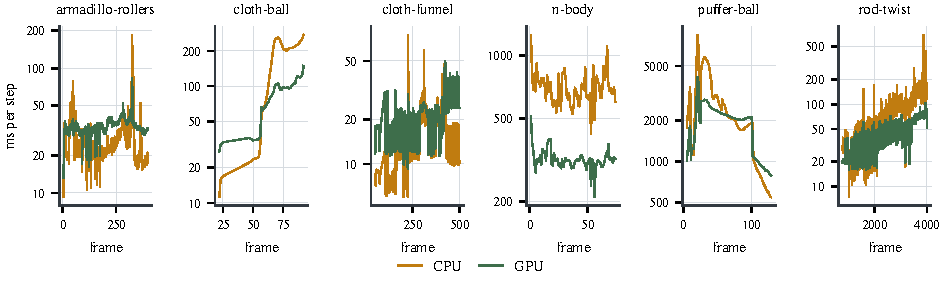
\includegraphics[width=\linewidth]{figures/per-frame.pdf}
  \caption{Per-frame cost of the whole pipeline, BP full plus NP EToI, in
    milliseconds for one simulation step, both query types together, against
    frame index. On cloth-funnel the device is behind for most of the
    trajectory, so its deficit is a standing gap and not a few expensive frames;
    on rod-twist the cost climbs steadily on both processors as the rod winds
    up, so the median understates the end of the simulation.}
  \label{fig:perframe}
\end{figure}

\begin{figure}[htbp]
  \centering
  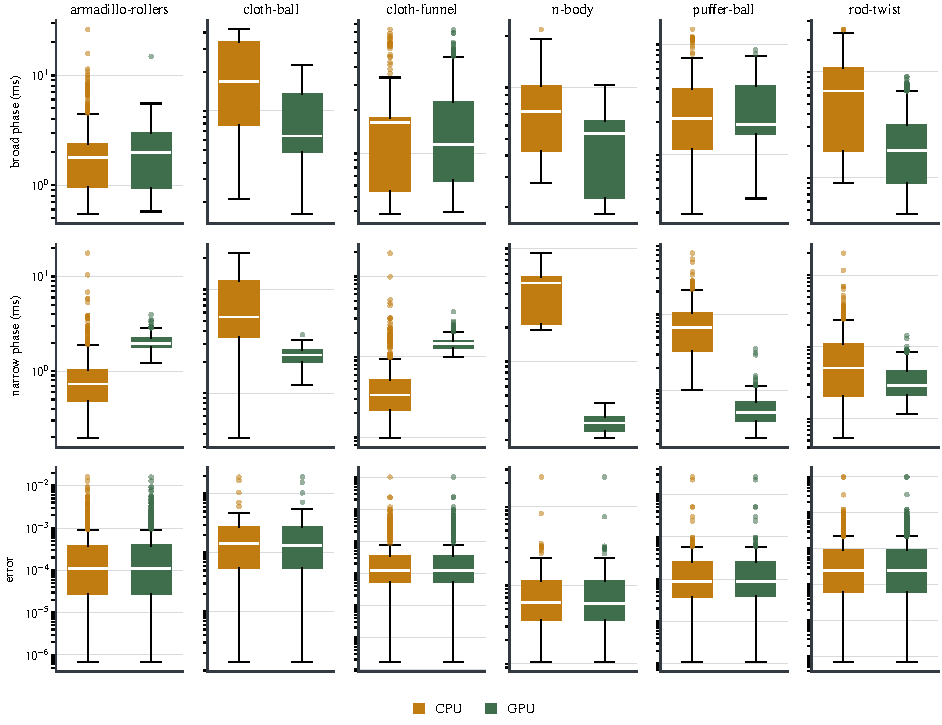
\includegraphics[width=\linewidth]{figures/results-grid.pdf}
  \caption{Per-case distributions over the six scenes, BP full above and NP
    EToI below. Each row shares one logarithmic scale, so a box is comparable
    across scenes as well as within one. Each box spans the first to the third
    quartile with the median inside, whiskers reach the furthest case within
    $1.5$ interquartile ranges, and cases beyond are drawn individually.
    Broad-phase time is tight around its median; narrow-phase time is skewed by
    a long upper tail.}
  \label{fig:grid}
\end{figure}

\begin{figure}[htbp]
  \centering
  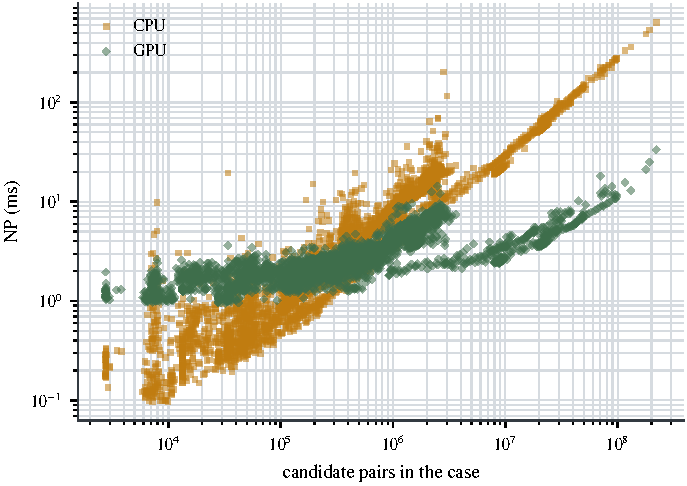
\includegraphics[width=0.78\linewidth]{figures/narrow-per-case.pdf}
  \caption{Per-case narrow-phase time against the number of candidate pairs in
    that case, over every case of every scene.}
  \label{fig:percase}
\end{figure}

\section{Scaling with thread count}
\label{sec:supp:threads}

The curves are plotted in \cref{fig:strong} of the article; this section gives
them scene by scene, over the same four cases at one to seventy-two Grace cores.
The queries scale well on both scenes, reaching $32.0\times$ on cloth-funnel and
$30.8\times$ on armadillo-rollers at seventy-two cores, as does the narrow
phase, at $17.0\times$ and $40.4\times$. Building the acceleration structure
limits the scaling: it reaches $4.0\times$ on cloth-funnel and $5.9\times$ on
armadillo-rollers at thirty-two cores and no further, $3.5\times$ and
$5.0\times$ at seventy-two, where the queries beside it are above $30$. A
component taking $8$ to $13\%$ of the single-core time therefore takes $38$ to
$48\%$ of it at seventy-two cores, and it holds the pipeline to $13.2\times$ and
$24.0\times$.

Three passes over every box account for the plateau, and all three are
reductions or histograms whose parallel forms are standard: the centre-variance
reduction that picks the two grid axes, the extent and mean reduction that sizes
the grid, and the counting histogram that fills it. What remains once they are
parallel is a floor: at seventy-two cores the structure pass costs about the
same per case whatever that case carries, so the residue is a fixed cost per
call and not a share of the work.

Between sixty-four and seventy-two cores the curves are flat, the queries and
the structure pass losing a few percent and the narrow phase gaining a little on
both scenes, so the figures above do not depend on which of the two thread
counts they are quoted at.

\section{The TightInclusion comparison, per scene}
\label{sec:supp:reference}

\Cref{tab:reference} carries the per-scene-phase form of the comparison the
article summarises per scene: queries, hits and time for each processor beside
the reference. \Cref{tab:earliness-ref} is the accuracy half, the earliness
statistics the article reports as identical on the host and close on the device.
Read per scene-phase the cost spans a wider range than the article's per-scene
totals do, from $1.7\times$ to $4.9\times$ on the host and $2.5\times$ to
$26.6\times$ on the device, since the two query types of one scene can differ by
more than the scenes do.

\begin{table}[htbp]
  \centering
  \caption{SCCD against TightInclusion over the same queries: hits reported, and time taken. TightInclusion is the reference implementation of a certified conservative narrow phase, so matching its hit count is the strongest agreement available; reporting more hits is a false positive, which costs work but is never unsafe.}
  \label{tab:reference}
  \fittable{%
  \begin{tabular}{lllrrrr}
    \toprule
    scene & phase & mode & queries & hits & time (ms) & vs.\ TI \\
    \midrule
    armadillo-rollers & EE & GPU & 99,104 & 98,761 & 2345 / 2361 & 4.3× \\
    armadillo-rollers & EE & CPU & 99,104 & 98,761 & 5865 / 5870 & 1.7× \\
    armadillo-rollers & EE & TightInclusion & 99,104 & 98,761 & 10113 / 10133 & 1.0× (ref) \\
    armadillo-rollers & VF & GPU & 32,337 & 32,122 & 1626 / 1635 & 4.4× \\
    armadillo-rollers & VF & CPU & 32,337 & 32,122 & 2473 / 2483 & 2.9× \\
    armadillo-rollers & VF & TightInclusion & 32,337 & 32,122 & 7231 / 7231 & 1.0× (ref) \\
    cloth-ball & EE & GPU & 557,683 & 557,668 & 491 / 495 & 5.4× \\
    cloth-ball & EE & CPU & 557,683 & 557,668 & 1037 / 1038 & 2.6× \\
    cloth-ball & EE & TightInclusion & 557,683 & 557,668 & 2655 / 2655 & 1.0× (ref) \\
    cloth-ball & VF & GPU & 107,257 & 107,252 & 341 / 342 & 3.8× \\
    cloth-ball & VF & CPU & 107,257 & 107,252 & 399 / 400 & 3.2× \\
    cloth-ball & VF & TightInclusion & 107,257 & 107,252 & 1280 / 1281 & 1.0× (ref) \\
    cloth-funnel & EE & GPU & 6,751 & 6,259 & 1135 / 1149 & 2.5× \\
    cloth-funnel & EE & CPU & 6,751 & 6,259 & 1262 / 1286 & 2.3× \\
    cloth-funnel & EE & TightInclusion & 6,751 & 6,259 & 2874 / 2935 & 1.0× (ref) \\
    cloth-funnel & VF & GPU & 801 & 529 & 416 / 421 & 2.9× \\
    cloth-funnel & VF & CPU & 801 & 529 & 243 / 244 & 4.9× \\
    cloth-funnel & VF & TightInclusion & 801 & 529 & 1197 / 1199 & 1.0× (ref) \\
    n-body & EE & GPU & 2,399,812 & 2,399,746 & 877 / 879 & 5.8× \\
    n-body & EE & CPU & 2,399,812 & 2,399,746 & 1501 / 1504 & 3.4× \\
    n-body & EE & TightInclusion & 2,399,812 & 2,399,746 & 5094 / 5111 & 1.0× (ref) \\
    n-body & VF & GPU & 547,907 & 547,874 & 631 / 645 & 3.0× \\
    n-body & VF & CPU & 547,907 & 547,873 & 479 / 479 & 4.0× \\
    n-body & VF & TightInclusion & 547,907 & 547,873 & 1911 / 1914 & 1.0× (ref) \\
    puffer-ball & EE & GPU & 1,206,952 & 1,187,650 & 919 / 922 & 4.3× \\
    puffer-ball & EE & CPU & 1,206,952 & 1,187,650 & 1713 / 1737 & 2.3× \\
    puffer-ball & EE & TightInclusion & 1,206,952 & 1,187,650 & 3958 / 3998 & 1.0× (ref) \\
    puffer-ball & VF & GPU & 307,220 & 299,698 & 625 / 626 & 2.8× \\
    puffer-ball & VF & CPU & 307,220 & 299,676 & 543 / 547 & 3.2× \\
    puffer-ball & VF & TightInclusion & 307,220 & 299,676 & 1733 / 1747 & 1.0× (ref) \\
    rod-twist & EE & GPU & 492,120 & 246,132 & 16253 / 16296 & 26.6× \\
    rod-twist & EE & CPU & 492,120 & 246,132 & 202624 / 202792 & 2.1× \\
    rod-twist & EE & TightInclusion & 492,120 & 246,132 & 432019 / 432263 & 1.0× (ref) \\
    rod-twist & VF & GPU & 57,088 & 40,544 & 8038 / 8137 & 9.4× \\
    rod-twist & VF & CPU & 57,088 & 40,542 & 18672 / 18773 & 4.1× \\
    rod-twist & VF & TightInclusion & 57,088 & 40,542 & 75762 / 75815 & 1.0× (ref) \\
    \bottomrule
  \end{tabular}}
  \par\smallskip\footnotesize Source: \texttt{benchmark/results/oracle-gh200-all.csv}
\end{table}


\begin{table}[htbp]
  \centering
  \caption{Earliness against the dataset's exact symbolic roots: how far before the true time of impact each implementation reports, as the median over files of the within-file median, and the largest anywhere in the scene. TightInclusion is a subject here rather than the reference, because its own answer is a conservative lower bound and not the truth.}
  \label{tab:earliness-ref}
  \fittable{%
  \begin{tabular}{lllrr}
    \toprule
    scene & phase & mode & median & worst case \\
    \midrule
    armadillo-rollers & EE & CPU & 3.11e-06 & 1.60e-02 \\
    armadillo-rollers & EE & GPU & 3.11e-06 & 1.60e-02 \\
    armadillo-rollers & EE & TightInclusion & 3.11e-06 & 1.60e-02 \\
    armadillo-rollers & VF & CPU & 3.74e-06 & 9.39e-03 \\
    armadillo-rollers & VF & GPU & 3.74e-06 & 9.39e-03 \\
    armadillo-rollers & VF & TightInclusion & 3.74e-06 & 9.39e-03 \\
    cloth-ball & EE & CPU & 1.05e-07 & 1.04e-04 \\
    cloth-ball & EE & GPU & 1.05e-07 & 1.04e-04 \\
    cloth-ball & EE & TightInclusion & 1.05e-07 & 1.04e-04 \\
    cloth-ball & VF & CPU & 9.76e-08 & 2.88e-05 \\
    cloth-ball & VF & GPU & 9.75e-08 & 2.75e-05 \\
    cloth-ball & VF & TightInclusion & 9.76e-08 & 2.88e-05 \\
    cloth-funnel & EE & CPU & 0 & 1.00e+00 \\
    cloth-funnel & EE & GPU & 0 & 1.00e+00 \\
    cloth-funnel & EE & TightInclusion & 0 & 1.00e+00 \\
    cloth-funnel & VF & CPU & 3.33e-04 & 2.67e-02 \\
    cloth-funnel & VF & GPU & 3.33e-04 & 2.67e-02 \\
    cloth-funnel & VF & TightInclusion & 3.33e-04 & 2.67e-02 \\
    n-body & EE & CPU & 1.14e-08 & 1.89e-04 \\
    n-body & EE & GPU & 1.14e-08 & 1.91e-04 \\
    n-body & EE & TightInclusion & 1.14e-08 & 1.89e-04 \\
    n-body & VF & CPU & 1.17e-08 & 1.87e-05 \\
    n-body & VF & GPU & 1.17e-08 & 1.87e-05 \\
    n-body & VF & TightInclusion & 1.17e-08 & 1.87e-05 \\
    puffer-ball & EE & CPU & 3.54e-05 & 2.61e-01 \\
    puffer-ball & EE & GPU & 3.54e-05 & 2.61e-01 \\
    puffer-ball & EE & TightInclusion & 3.54e-05 & 2.61e-01 \\
    puffer-ball & VF & CPU & 4.58e-05 & 5.04e-02 \\
    puffer-ball & VF & GPU & 4.56e-05 & 5.05e-02 \\
    puffer-ball & VF & TightInclusion & 4.58e-05 & 5.04e-02 \\
    rod-twist & EE & CPU & 3.69e-04 & 9.85e-01 \\
    rod-twist & EE & GPU & 3.68e-04 & 9.85e-01 \\
    rod-twist & EE & TightInclusion & 3.69e-04 & 9.85e-01 \\
    rod-twist & VF & CPU & 1.54e-04 & 9.93e-01 \\
    rod-twist & VF & GPU & 1.55e-04 & 9.93e-01 \\
    rod-twist & VF & TightInclusion & 1.54e-04 & 9.93e-01 \\
    \bottomrule
  \end{tabular}}
  \par\smallskip\footnotesize Source: \texttt{benchmark/assessment/broadphase-cell2dmin.csv}
\end{table}


\section{The competitor comparisons, per scene}
\label{sec:supp:competitors}

\Cref{tab:competitor-earliest,tab:competitor-pair} carry the per-scene numbers
the article summarises. Beyond the cost columns they hold the accuracy columns:
the earliness statistics, the count of steps answered after the root, and the
false positives.

\begin{table}[htbp]
  \centering
  \caption{Earliest time of impact per simulation step, against Scalable
    CCD~\citep{belgrod2025toi}. Both libraries run their
    earliest-time-of-impact path once per case from a bound of $1$, over
    identical broad-phase candidates, and a step's answer is the minimum over
    its cases. \emph{earliness} is the step's earliest exact root minus the
    answer reported for it, so a positive value is conservative and a negative
    one is an answer after the root; \emph{late} counts the steps where it is
    negative, per pass over the case list. \emph{total} is the whole scene,
    prep and broad phase and narrow phase together, summed over every case with
    the median over repeats taken first; \emph{avg} divides it by the cases of
    the scene.}
  \label{tab:competitor-earliest}
  \fittable{%
\begin{tabular}{llrrrrr}
    \toprule
    scene & library & earl.\ med. & earl.\ max & late & total (ms) & avg (ms) \\
    \midrule
    armadillo-rollers & SCCD (CPU) & 1.24e-06 & 0.00144 & 0 & 4,988 & 6.39 \\
     & SCCD (GPU) & 1.32e-06 & 0.00144 & 0 & 4,399 & 5.63 \\
     & Scalable CCD (GPU) & -0.00892 & 0.0883 & 265 & 15,419 & 19.74 \\
    \midrule
    cloth-ball & SCCD (CPU) & 1.66e-07 & 3.23e-06 & 0 & 2,438 & 30.86 \\
     & SCCD (GPU) & 1.69e-07 & 5.84e-06 & 0 & 1,220 & 15.44 \\
     & Scalable CCD (GPU) & 9.97e-06 & 0.931 & 0 & 5,510 & 69.75 \\
    \midrule
    cloth-funnel & SCCD (CPU) & 0 & 0.0167 & 0 & 2,886 & 5.00 \\
     & SCCD (GPU) & 0 & 0.0167 & 0 & 2,674 & 4.64 \\
     & Scalable CCD (GPU) & 0 & 0.963 & 8 & 10,025 & 17.37 \\
    \midrule
    n-body & SCCD (CPU) & 0 & 0 & 0 & 17,623 & 120.70 \\
     & SCCD (GPU) & 0 & 0 & 0 & 7,827 & 53.61 \\
     & Scalable CCD (GPU) & 0 & 0 & 0 & 30,292 & 207.48 \\
    \midrule
    puffer-ball & SCCD (CPU) & 1.76e-05 & 0.000315 & 0 & 462,900 & 1928.75 \\
     & SCCD (GPU) & 1.85e-05 & 0.000315 & 0 & 75,312 & 313.80 \\
     & Scalable CCD (GPU) & 0.0584 & 0.925 & 0 & 278,643 & 1161.01 \\
    \midrule
    rod-twist & SCCD (CPU) & 7.32e-05 & 0.286 & 0 & 77,975 & 17.06 \\
     & SCCD (GPU) & 7.23e-05 & 0.286 & 0 & 44,546 & 9.75 \\
     & Scalable CCD (GPU) & 0.0203 & 0.706 & 33 & 143,094 & 31.30 \\
    \bottomrule
  \end{tabular}}
  \par\smallskip\footnotesize Scalable CCD's narrow phase is CUDA only, so it has
  no CPU row; its host broad phase is discussed in the text.
  \par\smallskip\footnotesize Some steps begin with their primitives already
  touching, so their earliest exact root is $0$ and every correct answer for them
  is $0$: cloth-funnel 272 of 363, n-body 74 of 74. Those steps hold the earliness columns at $0$
  without saying anything about tightness.
  \par\smallskip\footnotesize Source: \texttt{benchmark/competitors/results/}
\end{table}


\begin{table}[htbp]
  \centering
  \caption{Per collision pair, against additive CCD~\citep{li2021codim} as the
    IPC toolkit implements it. Both narrow phases are timed over the same
    broad-phase candidates -- additive CCD answers one pair at a time and carries
    no parallelism of its own, so it is driven by the parallel loop the toolkit's
    own stepsize query uses, on the same $72$ threads -- and both are scored on
    every curated query at the coordinates its exact root was computed for.
    \emph{f.p.} and \emph{missed} are counts per pass over the case list.
    \emph{earliness} is the query's exact root minus the time of impact
    reported for it, so a positive value is conservative, and no query of either library is answered after its root.
    \emph{total} is the narrow phase over the whole scene, summed over every case with the median
    over repeats taken first, and \emph{avg} divides it by the candidates it
    was handed. \emph{slowdown} is our total over additive CCD's, so above one
    is what the tighter answer costs, and \emph{tighter} is its median
    earliness over ours, so above one is how many times further from the root its
    median answer sits.}
  \label{tab:competitor-pair}
  \fittable{%
\begin{tabular}{llrrrrrrrr}
    \toprule
    scene & library & f.p. & missed & earl.\ med. & earl.\ max & total (ms) & avg (ns/pair) & slowdown & tighter \\
    \midrule
    armadillo-rollers & SCCD (CPU) & 24 & 0 & 3.39e-06 & 0.016 & 2,773 & 32.5 & 4.95$\times$ & 8,436$\times$ \\
     & SCCD (GPU) & 24 & 0 & 3.41e-06 & 0.016 & 2,669 & 31.3 & 4.77$\times$ & 8,397$\times$ \\
     & Additive CCD (CPU) & 444 & 0 & 0.0286 & 0.996 & 559.9 & 6.56 & 1.0$\times$ (ref) & 1.0$\times$ (ref) \\
    \midrule
    cloth-ball & SCCD (CPU) & 1 & 0 & 2.72e-07 & 0.000193 & 1,616 & 9.23 & 6.68$\times$ & 241,276$\times$ \\
     & SCCD (GPU) & 1 & 0 & 2.7e-07 & 0.000193 & 856.9 & 4.89 & 3.54$\times$ & 242,827$\times$ \\
     & Additive CCD (CPU) & 21 & 0 & 0.0656 & 0.94 & 241.8 & 1.38 & 1.0$\times$ (ref) & 1.0$\times$ (ref) \\
    \midrule
    cloth-funnel & SCCD (CPU) & 15 & 0 & 6.87e-06 & 1 & 725.8 & 28.8 & 2.02$\times$ & 1,248$\times$ \\
     & SCCD (GPU) & 15 & 0 & 6.83e-06 & 1 & 1,055 & 41.9 & 2.94$\times$ & 1,256$\times$ \\
     & Additive CCD (CPU) & 422 & 0 & 0.00857 & 0.956 & 358.8 & 14.2 & 1.0$\times$ (ref) & 1.0$\times$ (ref) \\
    \midrule
    n-body & SCCD (CPU) & 11 & 0 & 3.02e-08 & 0.00024 & 20,459 & 9.08 & 6.28$\times$ & 2,128,613$\times$ \\
     & SCCD (GPU) & 12 & 0 & 3.02e-08 & 0.00024 & 4,351 & 1.93 & 1.34$\times$ & 2,132,148$\times$ \\
     & Additive CCD (CPU) & 107 & 0 & 0.0643 & 0.897 & 3,257 & 1.45 & 1.0$\times$ (ref) & 1.0$\times$ (ref) \\
    \midrule
    puffer-ball & SCCD (CPU) & 536 & 0 & 4e-05 & 0.261 & 41,620 & 5.68 & 4.65$\times$ & 2,624$\times$ \\
     & SCCD (GPU) & 558 & 0 & 4.03e-05 & 0.261 & 10,979 & 1.5 & 1.23$\times$ & 2,608$\times$ \\
     & Additive CCD (CPU) & 27374 & 0 & 0.105 & 0.976 & 8,943 & 1.22 & 1.0$\times$ (ref) & 1.0$\times$ (ref) \\
    \midrule
    rod-twist & SCCD (CPU) & 1243 & 0 & 0.000275 & 0.993 & 82,393 & 21.3 & 11.96$\times$ & 84.6$\times$ \\
     & SCCD (GPU) & 1245 & 0 & 0.000275 & 0.993 & 27,388 & 7.07 & 3.97$\times$ & 84.5$\times$ \\
     & Additive CCD (CPU) & 16708 & 0 & 0.0232 & 0.994 & 6,891 & 1.78 & 1.0$\times$ (ref) & 1.0$\times$ (ref) \\
    \bottomrule
  \end{tabular}}
  \par\smallskip\footnotesize Source: \texttt{benchmark/competitors/results/}
\end{table}


\section{The race in Scalable CCD's subdivision buffer}
\label{sec:supp:race}

The article reports that Scalable CCD answers after the true root on three
scenes. The cause is a race in its subdivision buffer, whose overflow check
tests that the buffer is full and then advances the tail as two separate
operations, so that concurrent pushes can wrap the tail onto domains that have
not been processed yet with no overflow flagged. Three observations identify it.
Padding a query list with pairs that fail their first inclusion test, which
changes nothing but the length of the list and hence the size the buffer is
given, turns $0$ of $1{,}299$ contacts found at one step into all $1{,}299$. The
answer differs between identical runs. A copy of the library whose overflow
check is made race-free finds every one of the $54{,}664$ curated contacts of
armadillo's first $400$ cases with nothing missed and nothing late. The article
reports the library as published; the patched copy is diagnosis only.

The set of affected scenes supports that reading. The buffer is sized from the
number of queries it is handed, so a short candidate list gives a small buffer:
the three scenes it fails are the three with the fewest candidate pairs per step,
and the three it answers correctly are those with millions.

\bibliographystyle{plainnat}
\bibliography{refs}

\end{document}
